\documentclass[12pt]{article}

\usepackage[table]{xcolor}

\usepackage[hidelinks]{hyperref}
\usepackage{etoolbox}
\usepackage{graphicx}
\usepackage{adjustbox}

\makeatletter
\def\ScaleIfNeeded{%
  \ifdim\Gin@nat@width>\linewidth
    \linewidth
  \else
    \Gin@nat@width
  \fi
}
\makeatother

% fonts
\usepackage[T1]{fontenc}
\usepackage[utf8]{inputenc}
\usepackage{textgreek}
\usepackage[greek,english]{babel}
\usepackage{amsmath}

% Code highlight and colors
\usepackage{listings}
\lstset{
  numbers=left,
  tabsize=1,
  basicstyle=\small\ttfamily,
  breaklines=true
}

\usepackage{booktabs, tabularx, longtable}
\usepackage{csquotes}
\usepackage{authblk}

% Geometry block
\usepackage[letterpaper]{geometry}
\providecommand{\tightlist}{\setlength{\itemsep}{0pt}\setlength{\parskip}{0pt}}

\title{Template for pandoc / markdown manuscripts}

\author[1,2]{Timothée~Poisot}
\author[2,3]{Second~Author}
\affil[1]{Université de Montréal, Département de Sciences Biologiques}
\affil[2]{Québec Centre for Biodiversity Sciences}
\affil[3]{University of Whatever}

\begin{document}

\maketitle

\begin{abstract}
  This template uses the magic of makefiles, pandoc, and markdown, to make
  it easy to produce multiple documents from markdown, R markdown, or
  Julia markdown files. Just type \lstinline!make! at the command line to
  see the different options.
\end{abstract}

<<<<<<< HEAD
=======
% pandoc-xnos: cleveref fakery
\newcommand{\plusnamesingular}{}
\newcommand{\starnamesingular}{}
\newcommand{\xrefname}[1]{\protect\renewcommand{\plusnamesingular}{#1}}
\newcommand{\Xrefname}[1]{\protect\renewcommand{\starnamesingular}{#1}}
\providecommand{\cref}{\plusnamesingular~\ref}
\providecommand{\Cref}{\starnamesingular~\ref}
\providecommand{\crefformat}[2]{}
\providecommand{\Crefformat}[2]{}

% pandoc-xnos: cleveref formatting
\crefformat{figure}{fig.~#2#1#3}
\Crefformat{figure}{Figure~#2#1#3}
\crefformat{table}{table~#2#1#3}
\Crefformat{table}{Table~#2#1#3}
\crefformat{equation}{eq.~#2#1#3}
\Crefformat{equation}{Equation~#2#1#3}

>>>>>>> b4c81ad06ea8cb76f643342400d46edf705d8cee
This project intends to make the generation of high-quality preprints
from markdown, R markdown, and Julia markdown documents easy. Once
downloaded, type \lstinline!make! to see the output. This will generate
two pdf documents and one OpenDocument file.

\section{Installation}\label{installation}

To get started, you will need the python \lstinline!pandoc-fignos!,
\lstinline!pandoc-eqnos!, and \lstinline!pandoc-tablenos! filters.

\begin{lstlisting}
make dependencies
\end{lstlisting}

Make sure that \lstinline!pandoc! and \lstinline!pandoc-citeproc! are
installed, and that you have a LaTeX installation. You will also need an
installation of node. If you want to use this template with reproducible
documents, you will need either \lstinline!knitr! or
\lstinline!Weave.jl!.

\section{Document options}\label{document-options}

There are two important files to edit to specificy the manuscript
informations. First, \lstinline!authors.yaml! should be
self-explanatory; it contains the author names, email addres for the
corresponding author, and affiliations. The \lstinline!infos.yaml! file
is for the manuscript title, keywords, etc. Finally, the
\lstinline!ABSTRACT! file has the abstract. It can contain markdown
formatting.

<<<<<<< HEAD
\section{Citations, tables, figures, \ldots{}}\label{sec:citation}

You can give sections identifiers with \lstinline!{#sec:id}!, and cite
them with \lstinline!@sec:id! -- for example, this is section
sec.~\ref{sec:citation}.
=======
\section{Citations, tables, figures,
\ldots{}}\label{citations-tables-figures}
>>>>>>> b4c81ad06ea8cb76f643342400d46edf705d8cee

\subsection{Tables}\label{tables}

Table legends go on the line after the table itself. To generate a
reference to the table, use \lstinline!{#tbl:id}! -- then, in the text,
you can use \lstinline!{@tbl:id}! to refer to the table. For example,
<<<<<<< HEAD
the table below is tbl.~\ref{tbl:id}. You can remove the \emph{table} in
front by using \lstinline"!@tbl:id", or force it to be capitalized with
\lstinline!\*tbl:id!.

\hypertarget{tbl:id}{}
\begin{longtable}[]{@{}lr@{}}
\caption{\label{tbl:id}This is a table, and its identifier is
\lstinline!id! -- we can refer to it using \lstinline!{@tbl:id}!. Note
that even if the table legend is written below the table itself, it will
appear on top in the compiled document. }\tabularnewline
=======
the table below is \xrefname{table}\cref{tbl:id}. You can remove the
\emph{table} in front by using \lstinline"!@tbl:id", or force it to be
capitalized with \lstinline!\*tbl:id!.

\begin{longtable}[]{@{}lr@{}}
\caption{This is a table, and its identifier is \lstinline!id! -- we can
refer to it using \lstinline!{@tbl:id}!. Note that even if the table
legend is written below the table itself, it will appear on top in the
compiled document. \label{tbl:id}}\tabularnewline
>>>>>>> b4c81ad06ea8cb76f643342400d46edf705d8cee
\toprule
Using & produces\tabularnewline
\midrule
\endfirsthead
\toprule
Using & produces\tabularnewline
\midrule
\endhead
<<<<<<< HEAD
\lstinline!@tbl:id! & tbl.~\ref{tbl:id}\tabularnewline
\lstinline"!@tbl:id" & !tbl.~\ref{tbl:id}\tabularnewline
\lstinline!\*@tbl:id! & *tbl.~\ref{tbl:id}\tabularnewline
=======
\lstinline!@tbl:id! & \xrefname{table}\cref{tbl:id}\tabularnewline
\lstinline"!@tbl:id" & \ref{tbl:id}\tabularnewline
\lstinline!\*@tbl:id! & \Xrefname{Table}\Cref{tbl:id}\tabularnewline
>>>>>>> b4c81ad06ea8cb76f643342400d46edf705d8cee
\bottomrule
\end{longtable}

\subsection{Equations}\label{equations}

Equations can be referenced using the same syntax as tables, using the
\lstinline!eq! prefix in place of \lstinline!tbl!. For example:

\begin{equation} y = mx + b \label{eq:id}\end{equation}

<<<<<<< HEAD
We can refer to eq.~\ref{eq:id} in the text.
=======
We can refer to \xrefname{eq.}\cref{eq:id} in the text.
>>>>>>> b4c81ad06ea8cb76f643342400d46edf705d8cee

\subsection{Adding references}\label{adding-references}

References go in the \lstinline!references.json! file, at the root of
the project. References are cited with \lstinline!@key!, where
\lstinline!key! is the unique identifier of the reference. Both inline,
like Hutchinson (1959), and in brackets (Hutchinson 1957) can be used.

\subsection{Figures}\label{figures}

Figures can be used with the usual markdown syntax. After the path, you
can use \lstinline!{#fig:id width=50%}! to specify the width and the
<<<<<<< HEAD
reference. See tbl.~\ref{tbl:id} for how to cite. The code below in the
markdown source produces fig.~\ref{fig:id}.

\begin{figure}
\centering
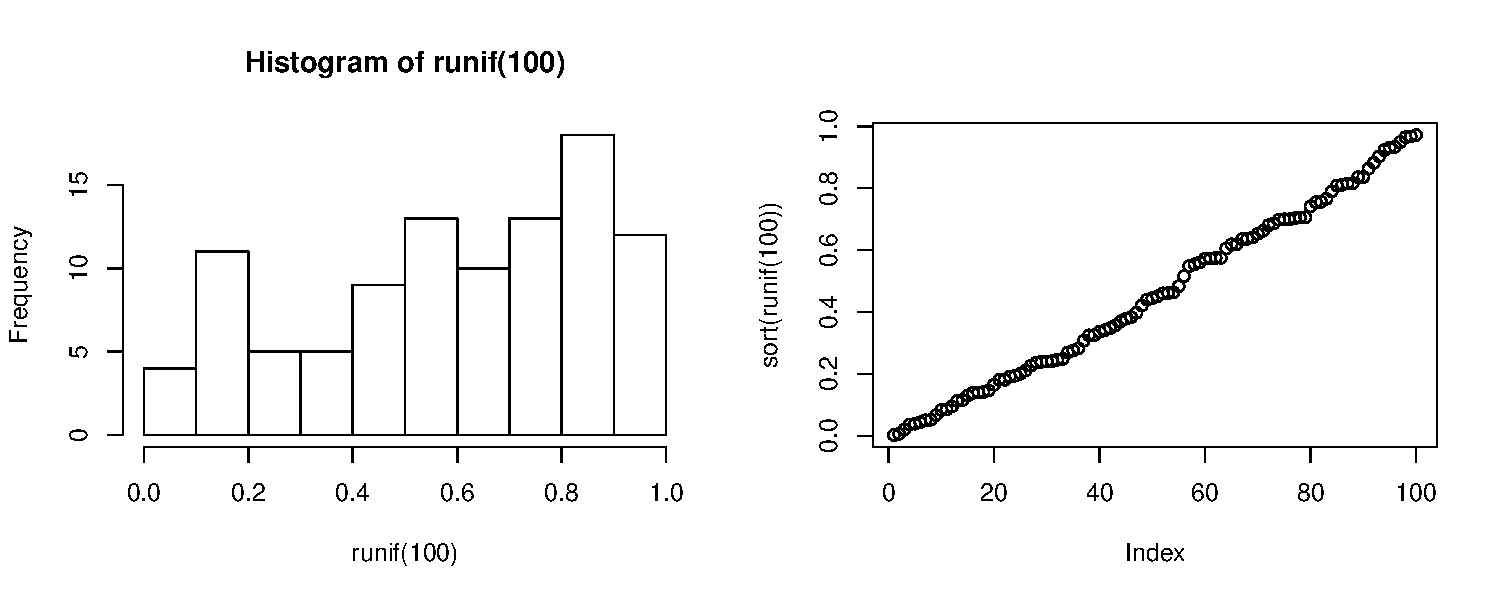
\includegraphics[width=1.00000\textwidth]{figure/histogram-1.pdf}
\caption{This is a figure. Figures can have identifiers, and the width
can be changed as well.}\label{fig:id}
=======
reference. See \xrefname{table}\cref{tbl:id} for how to cite. The code
below in the markdown source produces \xrefname{fig.}\cref{fig:id}.

\begin{figure}[htbp]
\centering
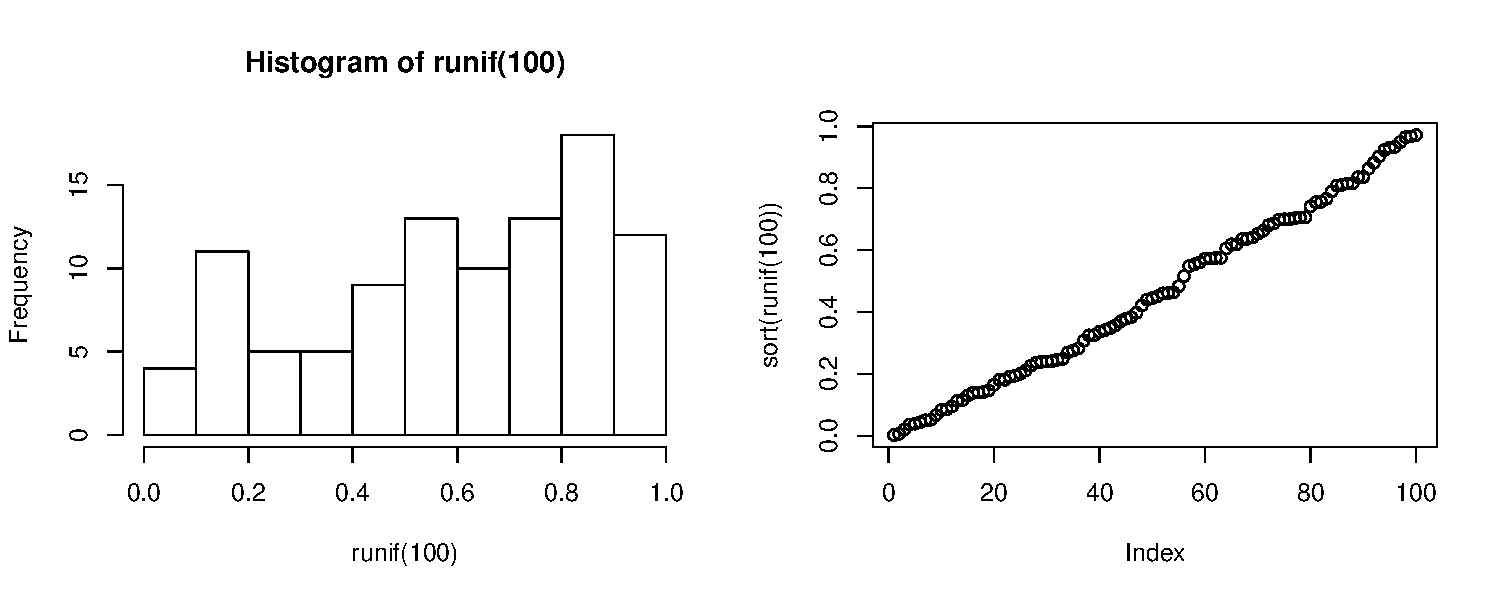
\includegraphics[width=1.00000\textwidth]{figure/histogram-1.pdf}
\caption{This is a figure. Figures can have identifiers, and the width
can be changed as well.\label{fig:id}}
>>>>>>> b4c81ad06ea8cb76f643342400d46edf705d8cee
\end{figure}

\section{Other elements}\label{other-elements}

\subsection{Code blocks}\label{code-blocks}

You can use fenced code blocks to render code:

\begin{lstlisting}
// Update affiliations
var print_affiliations = []
for (var af in affiliations) {
  var afobject = {}
  afobject.id = affiliations[af]
  afobject.text = af
  print_affiliations.push(afobject)
}
\end{lstlisting}

Note that code blocks have line numbers of the left, so this does not
interfer with the line numbers of the text (which are on the right).

\subsection{Track changes}\label{track-changes}

You can use \lstinline!make diff! to create a marked-up pdf document.
The git revision can be specified with the \lstinline!TAG! variable of
\lstinline!make! (by default, the latest commit). The other option is
\lstinline!AS!, which can be \lstinline!draft! or \lstinline!preprint!,
to render the marked-up version as a draft or as a preprint.

\subsection{Editorial marks}\label{editorial-marks}

\href{http://criticmarkup.com/}{Critic Markup} is rendered:

Don't go around saying\remove{to people that} the world owes you a
living. The world owes you nothing. It was here first.
\remove{One}\add{Only one} thing is impossible for God: To find
\add{any} sense in any copyright law on the planet.
\highlight{Truth is stranger than fiction}\note{strange but
true}, but it is because Fiction is obliged to stick to possibilities;
Truth isn't.

Note that CriticMarkup is \emph{not} rendered into OpenDocument.

\subsection{Using with knitr, Weave.jl,
\ldots{}}\label{using-with-knitr-weave.jl}

Just type \lstinline!make!. If there is a \lstinline!Rmd! or
\lstinline!Jmd! document with the same base name, the makefile will
render the markdown document for you. In fact, this document \emph{is} a
\lstinline!Rmd! file:

\begin{lstlisting}[language=R]
summary(rnorm(250))
\end{lstlisting}

\begin{lstlisting}
##      Min.   1st Qu.    Median      Mean   3rd Qu.      Max. 
<<<<<<< HEAD
## -2.723521 -0.712167 -0.007038 -0.049100  0.662052  3.038759
=======
## -2.900559 -0.645437 -0.033311  0.008348  0.670034  2.762948
>>>>>>> b4c81ad06ea8cb76f643342400d46edf705d8cee
\end{lstlisting}

Note that the extensions \emph{must} be \lstinline!Rmd! or
\lstinline!Jmd!, with an uppercase first letter. Of course you will need
\lstinline!knitr! (for \lstinline!R!) or \lstinline!Weave.jl! (for
\lstinline!julia!).

Because of the way figures are refered to (using the \lstinline!@fig:id!
syntax), it is better to generate the figure first, and then call it in
the text, using \lstinline!fig.show='hide'!. The code below will
<<<<<<< HEAD
generate fig.~\ref{fig:chunk}.
=======
generate \xrefname{fig.}\cref{fig:chunk}.
>>>>>>> b4c81ad06ea8cb76f643342400d46edf705d8cee

\begin{lstlisting}[language=R]
plot(sort(rnorm(200)), type='l')
\end{lstlisting}

You can then use this figure:

<<<<<<< HEAD
\begin{figure}
=======
\begin{figure}[htbp]
>>>>>>> b4c81ad06ea8cb76f643342400d46edf705d8cee
\centering
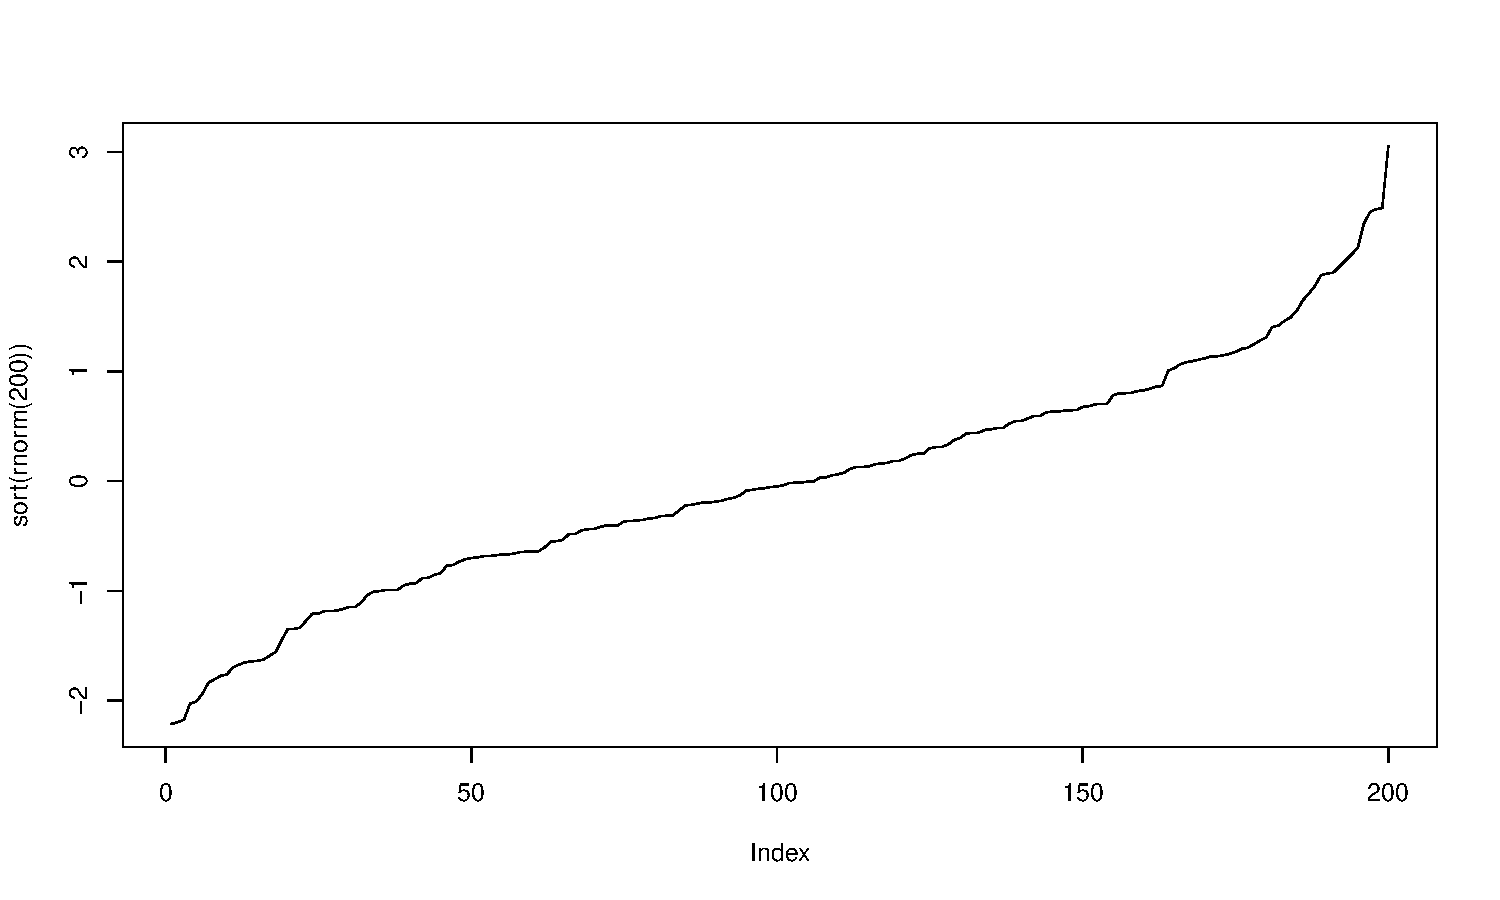
\includegraphics[width=1.00000\textwidth]{figure/testfig-1.pdf}
\caption{This is the figure created by the chunck \lstinline!testfig!,
so it is in \lstinline!figure/testfig-1!. You can use different
\lstinline!dev! in the knitr chunk options, so it is possible to
<<<<<<< HEAD
generate pdf or png figures.}\label{fig:chunk}
=======
generate pdf or png figures.\label{fig:chunk}}
>>>>>>> b4c81ad06ea8cb76f643342400d46edf705d8cee
\end{figure}

With \lstinline!knitr!, the \lstinline!kable! function can create
tables. If you add the caption paragraph immediately below, then these
<<<<<<< HEAD
tables can be cited. This is how we produce tbl.~\ref{tbl:knit}.
=======
tables can be cited. This is how we produce
\xrefname{table}\cref{tbl:knit}.
>>>>>>> b4c81ad06ea8cb76f643342400d46edf705d8cee

\begin{lstlisting}[language=R]
data(iris)
kable(head(iris))
\end{lstlisting}

<<<<<<< HEAD
\hypertarget{tbl:knit}{}
\begin{longtable}[]{@{}rrrrl@{}}
\caption{\label{tbl:knit}This is a table, and its identifier is
\lstinline!knit! -- we can refer to it using \lstinline!{@tbl:knit}!.
Note that even if the table legend is written below the table itself, it
will appear on top in the compiled document. }\tabularnewline
=======
\begin{longtable}[]{@{}rrrrl@{}}
\caption{This is a table, and its identifier is \lstinline!knit! -- we
can refer to it using \lstinline!{@tbl:knit}!. Note that even if the
table legend is written below the table itself, it will appear on top in
the compiled document. \label{tbl:knit}}\tabularnewline
>>>>>>> b4c81ad06ea8cb76f643342400d46edf705d8cee
\toprule
Sepal.Length & Sepal.Width & Petal.Length & Petal.Width &
Species\tabularnewline
\midrule
\endfirsthead
\toprule
Sepal.Length & Sepal.Width & Petal.Length & Petal.Width &
Species\tabularnewline
\midrule
\endhead
5.1 & 3.5 & 1.4 & 0.2 & setosa\tabularnewline
4.9 & 3.0 & 1.4 & 0.2 & setosa\tabularnewline
4.7 & 3.2 & 1.3 & 0.2 & setosa\tabularnewline
4.6 & 3.1 & 1.5 & 0.2 & setosa\tabularnewline
5.0 & 3.6 & 1.4 & 0.2 & setosa\tabularnewline
5.4 & 3.9 & 1.7 & 0.4 & setosa\tabularnewline
\bottomrule
\end{longtable}

\section*{References}\label{references}
\addcontentsline{toc}{section}{References}

\hypertarget{refs}{}
\hypertarget{ref-hutc57cr}{}
\textbf{Hutchinson}. (1957). Concluding remarks. \emph{Cold Spring Harb
Symp Quant Biol.} 22:415--27.

\hypertarget{ref-hutc59hsr}{}
\textbf{Hutchinson}. (1959). Homage to Santa Rosalia or why are there so
many kinds of animals? \emph{Am Nat.} 93:145.

\end{document}
